% !Mode:: "TeX:UTF-8"%確保文檔utf-8編碼
\documentclass[tikz,border=2pt]{standalone}
\usepackage{pgfplots}
\pgfplotsset{compat=newest}
\usetikzlibrary{decorations.pathreplacing}
\begin{document}
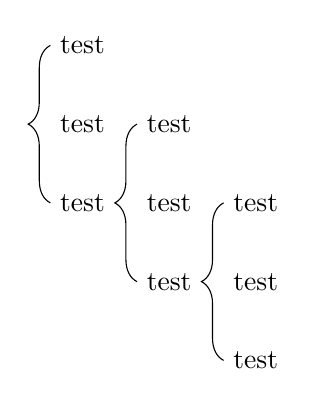
\begin{tikzpicture}
\draw [decorate,decoration={brace,amplitude=8}] (0,0) -- (0,2);
\node[right]  at (0,0) {test};
\node[right]  at (0,2) {test};
\node[right]  at (0,1) {test};

\begin{scope}[xshift=1.1cm,yshift=-1cm]
\draw [decorate,decoration={brace,amplitude=8}] (0,0) -- (0,2);
\node[right]  at (0,0) {test};
\node[right]  at (0,2) {test};
\node[right]  at (0,1) {test};
\end{scope}

\begin{scope}[xshift=2.2cm,yshift=-2cm]
\draw [decorate,decoration={brace,amplitude=8}] (0,0) -- (0,2);
\node[right]  at (0,0) {test};
\node[right]  at (0,2) {test};
\node[right]  at (0,1) {test};
\end{scope}

\end{tikzpicture}
\end{document}